\title{Final Exam for Algebra-Based Physics-1: Mechanics (PHYS135A-01)}
\author{Dr. Jordan Hanson - Whittier College Dept. of Physics and Astronomy}
\date{December 13th, 2017}
\documentclass[10pt]{article}
\usepackage[a4paper, total={18cm, 27cm}]{geometry}
\usepackage{outlines}
\usepackage[sfdefault]{FiraSans}
\usepackage{graphicx}

\begin{document}
\maketitle

\section{Conceptual Questions}
\subsection{Kinematics and Angular Kinematics}
\begin{enumerate}
\item If an object is dropped, it accelerates downward at $g$ m/s$^2$ (no air resistance).  If it is \textit{thrown} downward, the acceleration downward
\begin{itemize}
\item is less than $g$
\item is more than $g$
\item remains $g$
\end{itemize}
\item An object accelerates with constant acceleration.  The displacement versus time curve is quadratic.  The velocity versus time plot should be $\rule{1cm}{0.15mm}$ and the acceleration versus time plot should be $\rule{1cm}{0.15mm}$.
\begin{itemize}
\item quadratic, linear
\item linear, flat
\item flat, linear
\item linear, quadratic
\end{itemize}
\item An object experiences constant \textit{angular} acceleration.  The angular velocity is a $\rule{1cm}{0.15mm}$ function of time, and the net external torque is $\rule{1cm}{0.15mm}$.
\begin{itemize}
\item linear, constant
\item Iinear, zero
\item quadratic, constant
\item quadratic, zero
\end{itemize}
\item A battleship fires simultaneously two shells at enemy ships (Fig. \ref{fig:battle}).  If the shells follow the parabolic trajectories shown, which ship gets hit first?
\begin{itemize}
\item A
\item Both at the same time
\item B
\end{itemize}
\begin{figure}[hb]
\centering
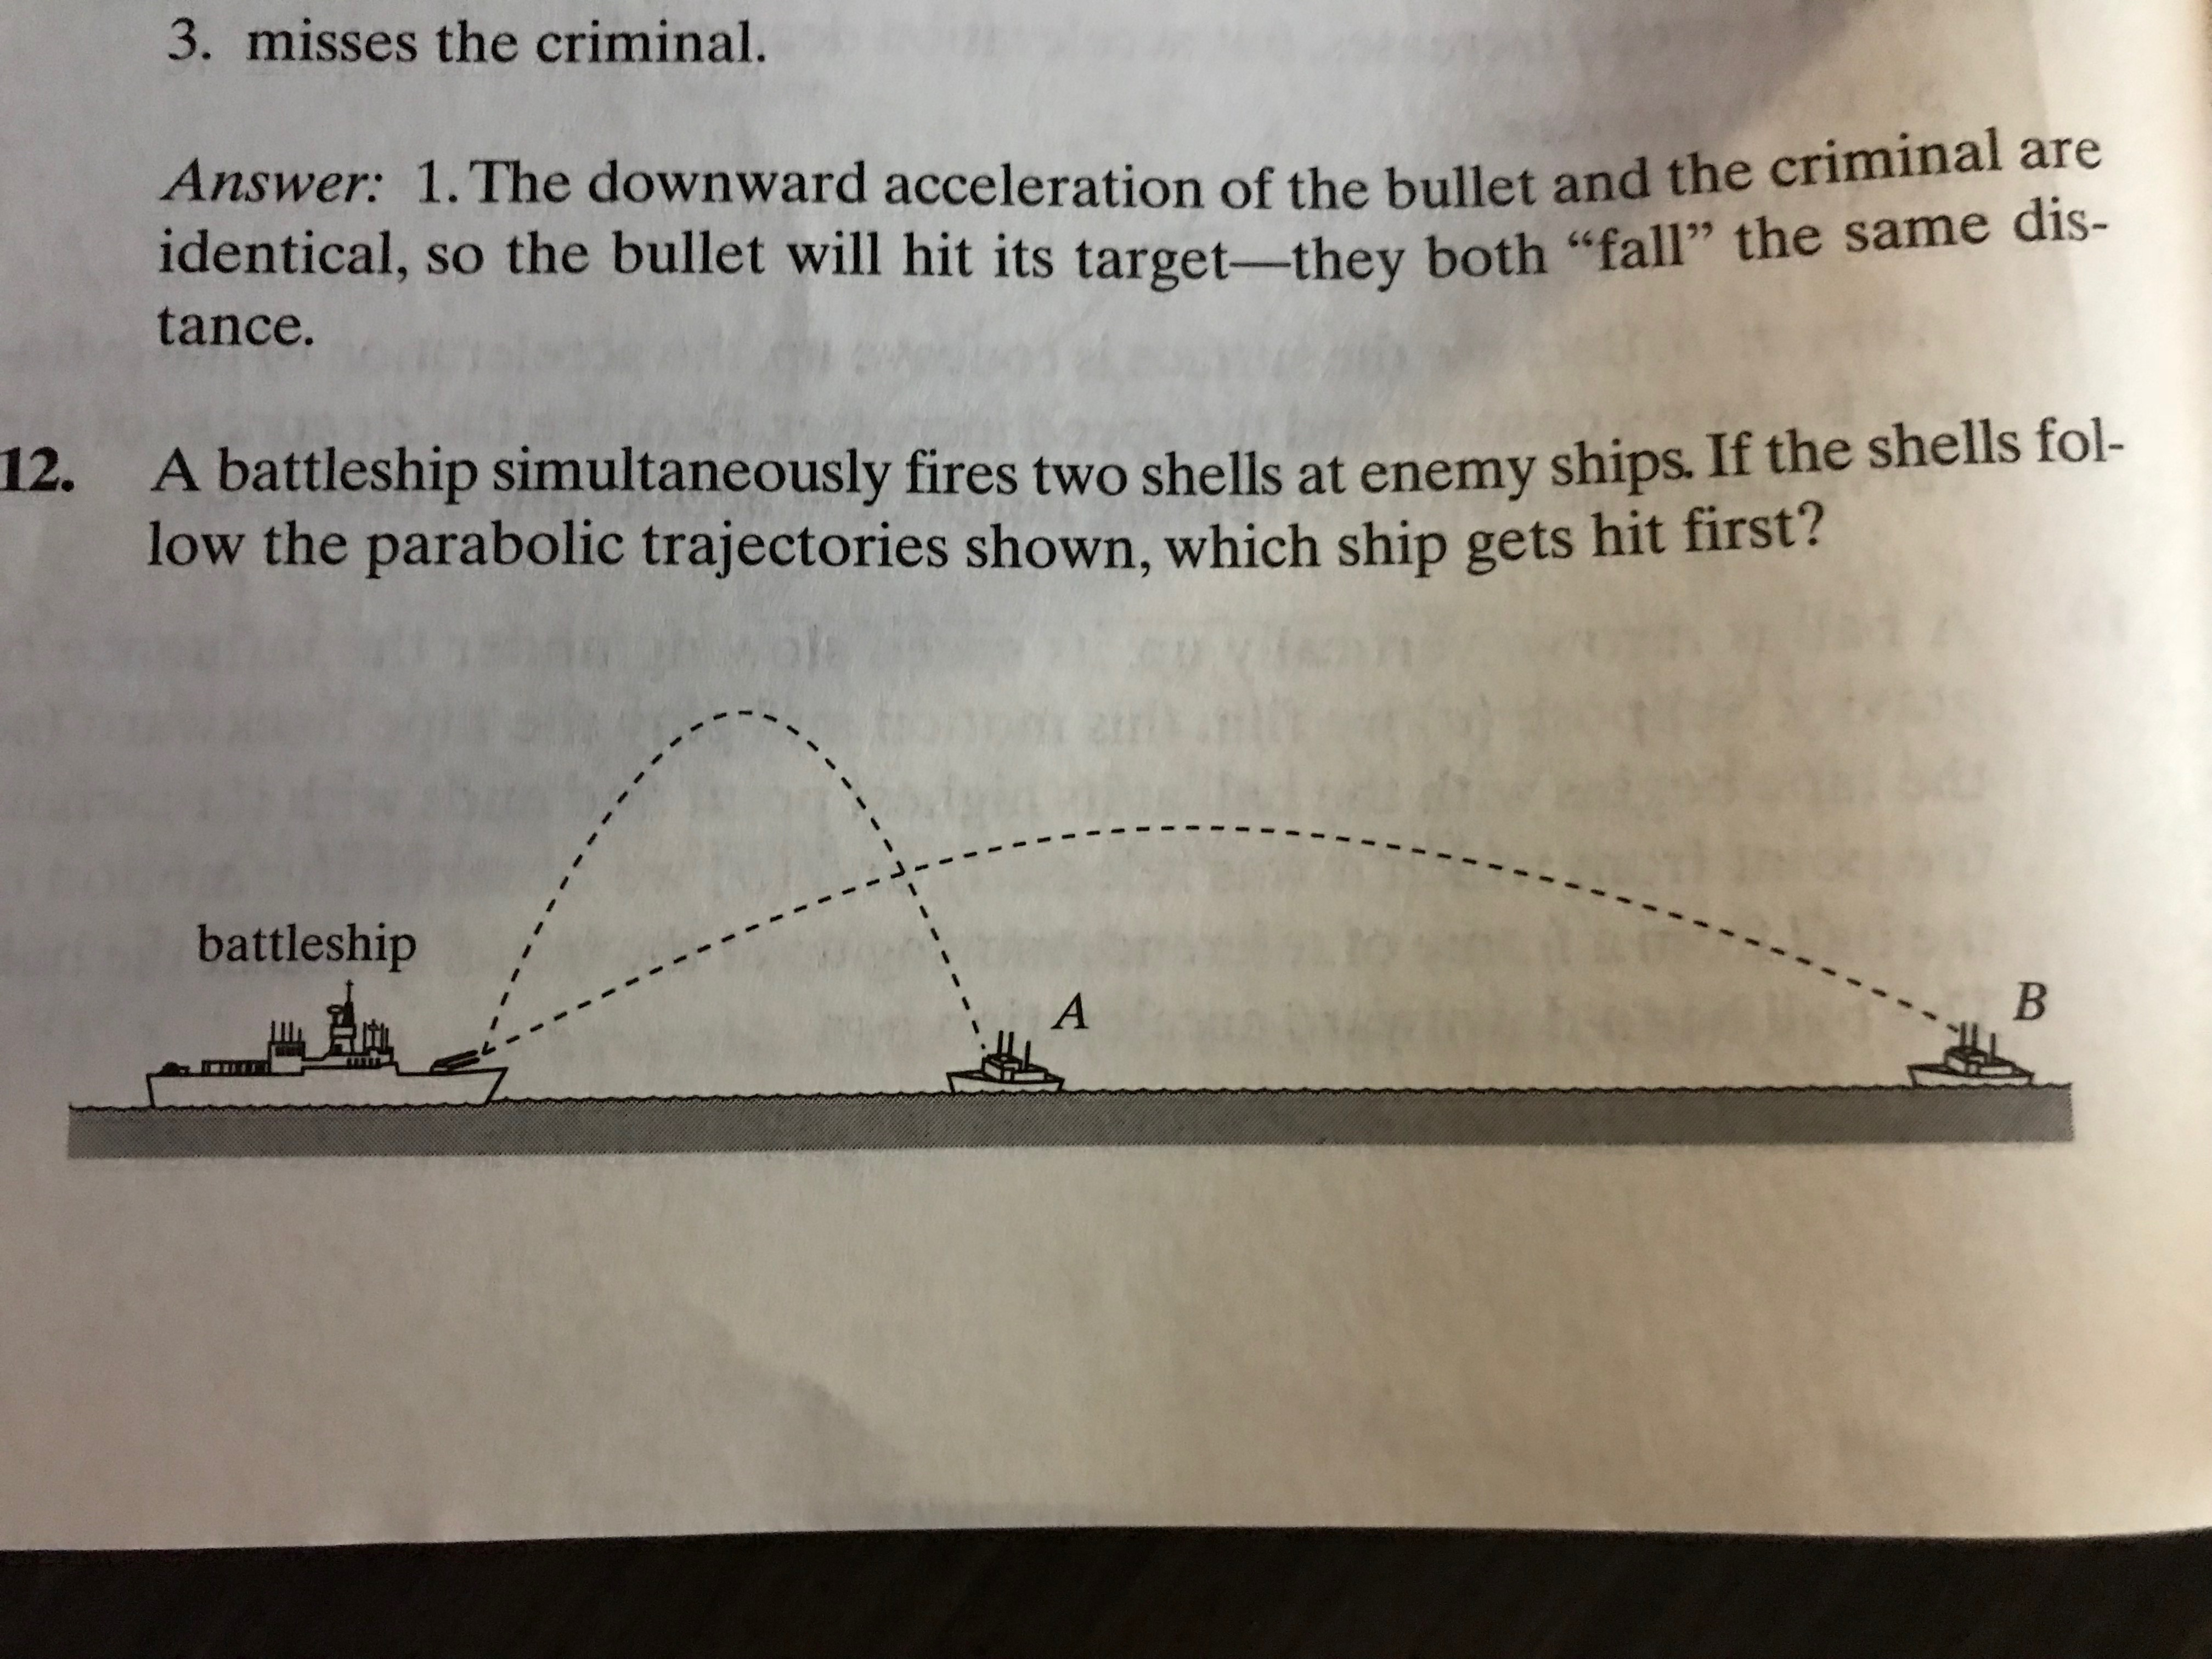
\includegraphics[width=0.6\textwidth,trim=0cm 30cm 0cm 45cm,clip=true]{battle.jpeg}
\caption{\label{fig:battle} Which ship is hit first?}
\end{figure}
\end{enumerate}
\subsection{Forces and Torque}
\begin{enumerate}
\item An elevator contains a person standing on a scale.  The elevator accelerates upward, then moves at constant velocity, then decelerates to a stop.  The scale reads a weight that is $\rule{1cm}{0.15mm}$, then $\rule{1cm}{0.15mm}$, and then $\rule{1cm}{0.15mm}$ the person's actual weight.
\begin{itemize}
\item More than, equal to, less than
\item Less than, equal to, more than
\item equal to, equal to, equal to
\item More than, equal to, equal to
\end{itemize}
\item A crate is pushed across a floor at constant velocity against friction.  If the crate is flipped so that a side with less surface area is on the bottom, and pushed again at constant velocity, the required force is
\begin{itemize}
\item More than the first side
\item Less than the first side
\item Equal to the first side
\end{itemize}
\item A man needs to pull a rusty lever to release a mechanism, but he can't.  Which of the following will increase torque on the lever?
\begin{itemize}
\item Tying a rope to the end of the lever, and pulling on the rope perpendicular to the lever.
\item Bolting a metal rod to the lever, and pulling the rod perpendicular to the lever.
\item Tying a rope to the end of the lever, pulling the rope parallel to the lever.
\item Bolting a metal rod to the lever, and pulling the rod parallel to the lever.
\end{itemize}
\item A racecar makes a turn at constant velocity, and the road is flat.  There is friction between the road and tires.  Which of the following is true?
\begin{itemize}
\item The car experiences centripetal acceleration, provided by friction.
\item The car experiences centripetal acceleration, provided by the normal force.
\item Moving at constant velocity, the car experiences no acceleration.
\end{itemize}
\end{enumerate}
\subsection{Work and Energy}
\begin{enumerate}
\item In which of the follow situations would energy \textit{not} be conserved?
\begin{itemize}
\item An object is dropped from some height and experiences free-fall, neglecting air-resistance.
\item An external force compresses a mass against an oscillator for a given displacement and then the mass is released.
\item A pendelum is pulled away from equilibrium and then released.
\item A rock slowly skids to a stop on top of a frozen pond.
\end{itemize}
\item A ball rolls down a hill that has a height $h$, attaining a speed $v$ at the bottom.  In order to attain a speed of $2v$ at the bottom, how tall would the hill have to be?
\begin{itemize}
\item $2h$
\item $3h$
\item $4h$
\end{itemize}
\end{enumerate}
\subsection{Linear and Angular Momentum}
\begin{enumerate}
\item A star undergoes a supernova, in which significant matter is blown away by a fusion reaction.  The remaining also shrinks in size.  Suppose the radius decreases by a factor of $10^3$.  By what factor does the angular velocity increase, if angular momentum is conserved? (Assume the mass doesn't change significantly).
\begin{itemize}
\item 10$^4$
\item 10$^5$
\item 10$^6$
\end{itemize}
\item A mine cart is moving along a track at constant speed, and passes under a vertical waterfall.  Because the cart is filled with water, the speed of the cart
\begin{itemize}
\item increases
\item decreases
\item remains constant (no net forces)
\end{itemize}
\item If ball 1 in the arrangement shown in Fig. \ref{fig:newton} is pulled back and then let go, ball 5 bounces forward.  If balls 1 and 2 are pulled back and released, balls 4 and 5 bounce forward, and so on.  The number of balls bouncing on each side is equal because
\begin{itemize}
\item of conservation of momentum.
\item the collisions are elastic.
\item the collisions are inelastic.
\item neither of the above.
\end{itemize}
\begin{figure}
\centering
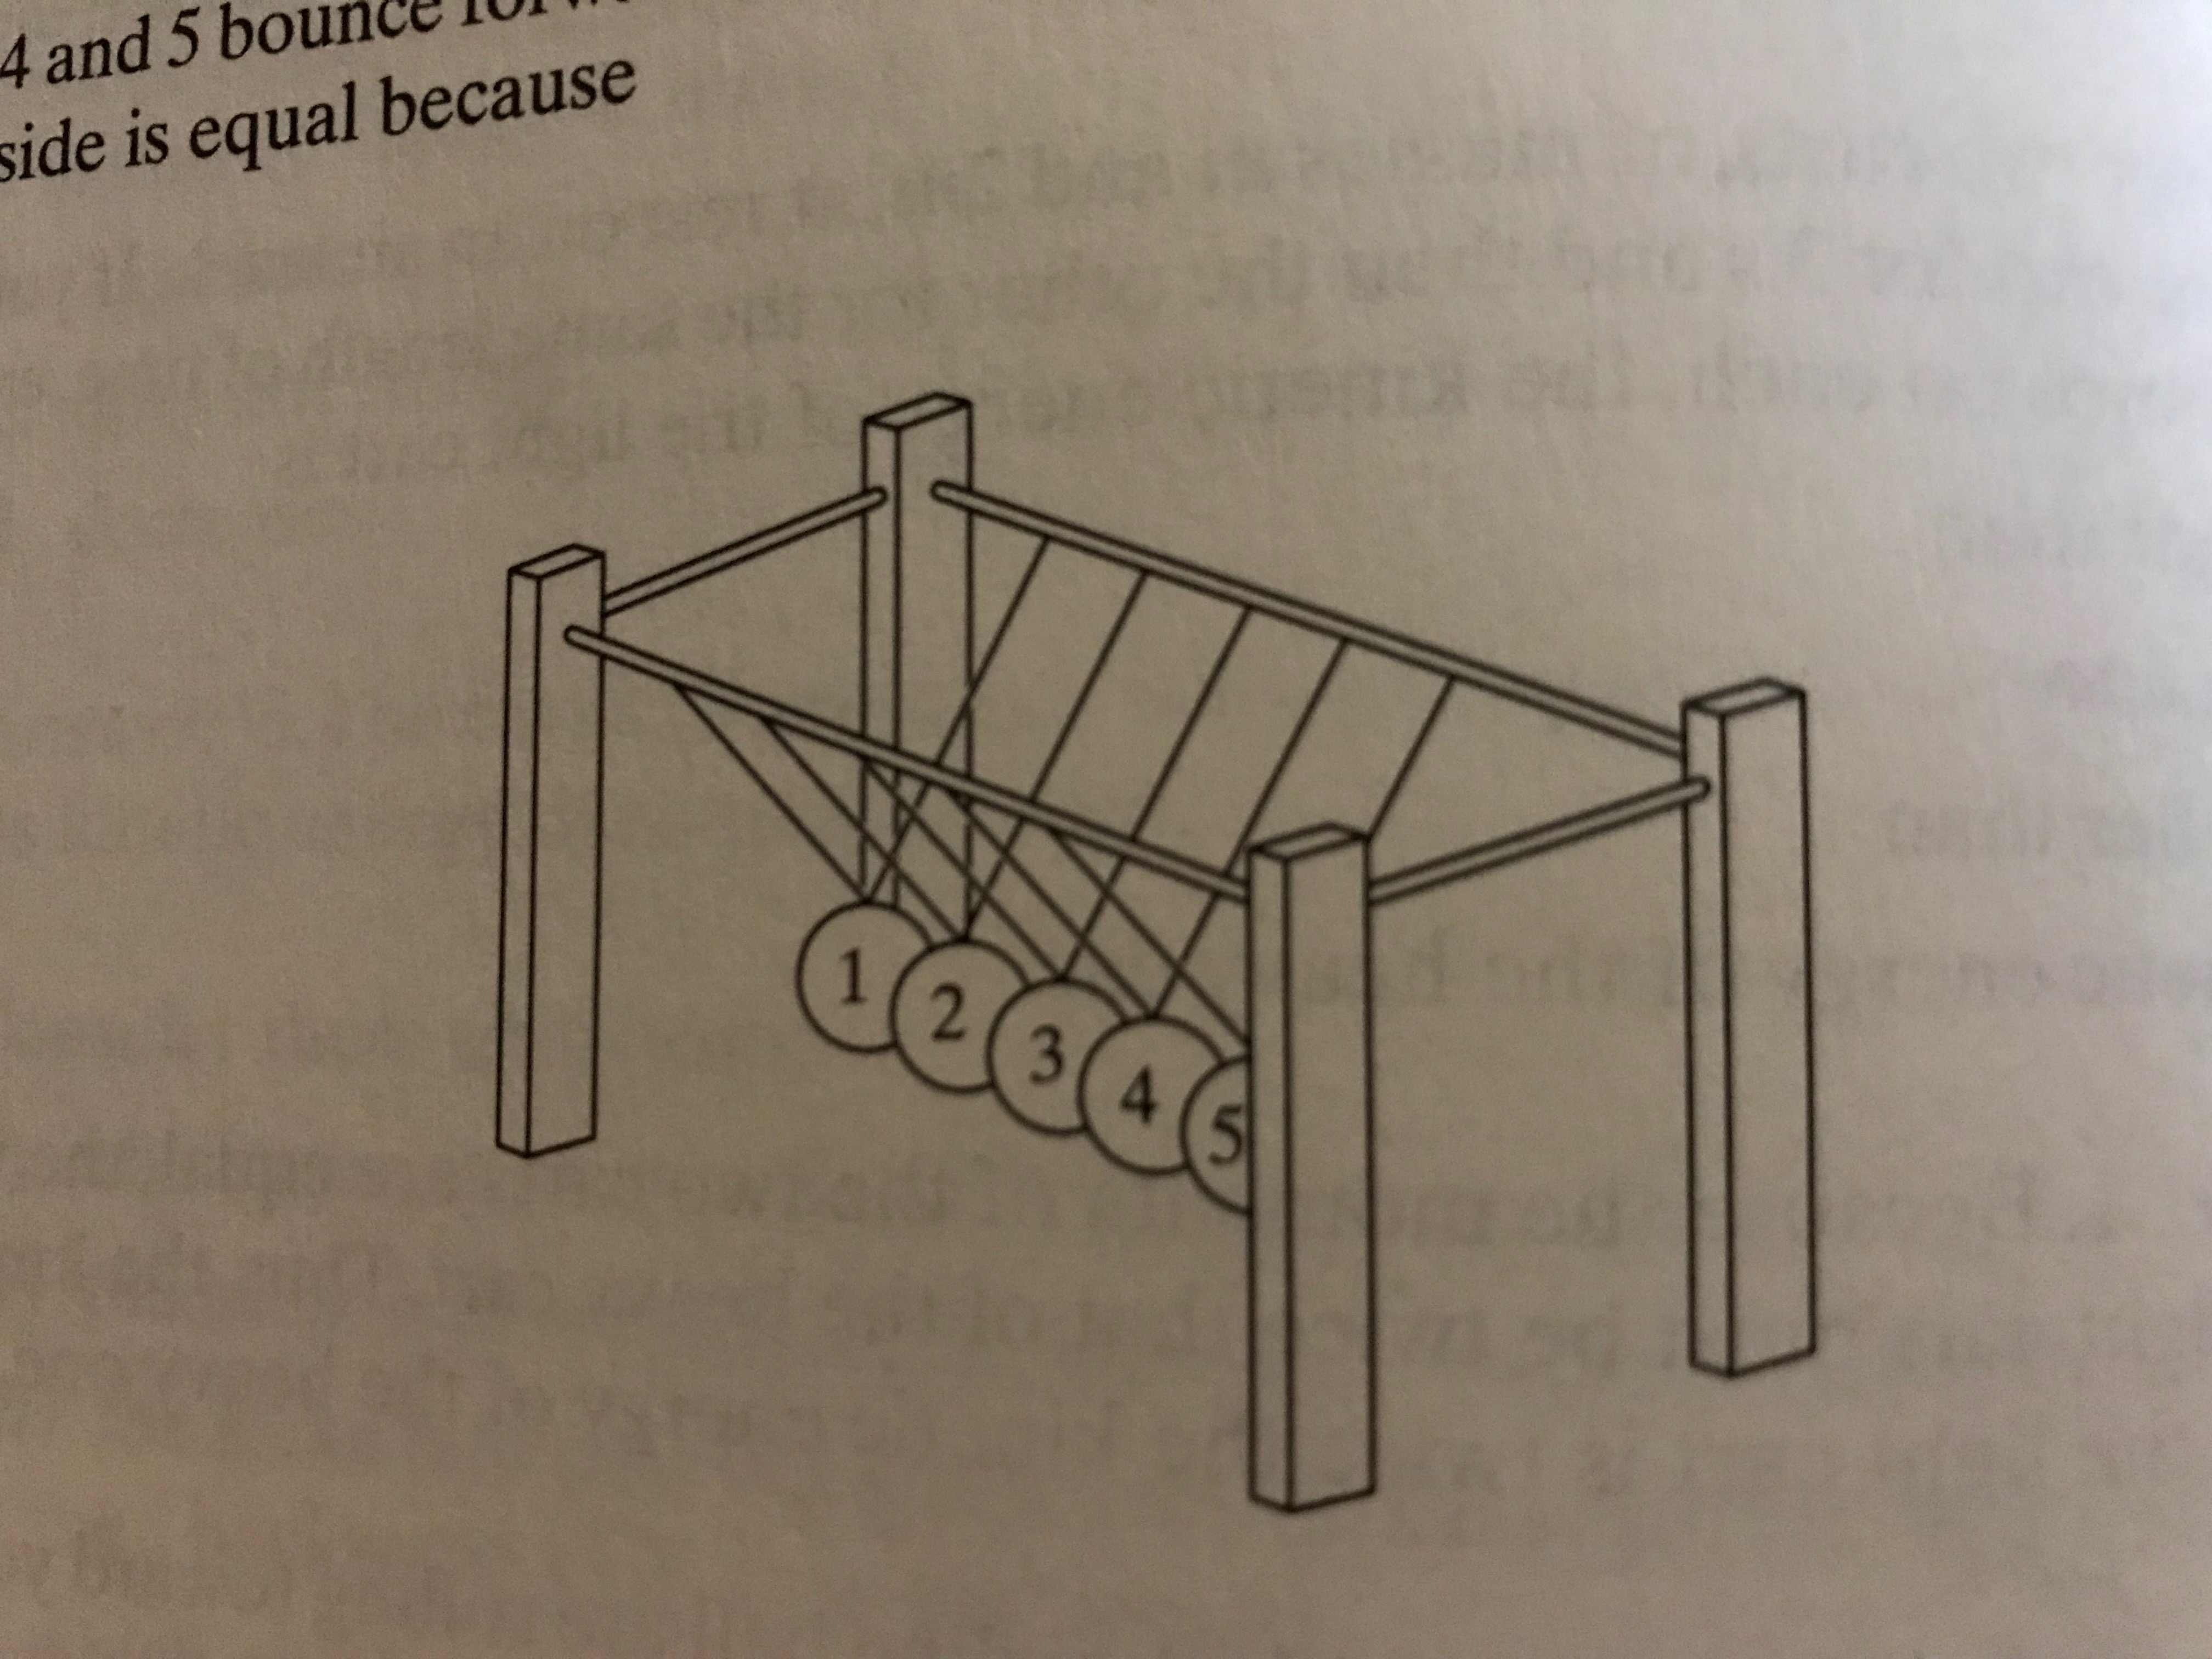
\includegraphics[width=0.2\textwidth,trim=20cm 5cm 15cm 20cm,clip=true]{newton.jpeg}
\caption{\label{fig:newton} This object is known as a Newton's cradle.}
\end{figure}
\end{enumerate}
\section{Technical Questions}
\subsection{Kinematics and Angular Kinematics}
\begin{enumerate}
\item A ball is kicked with an initial velocity of $\vec{v} = 4\hat{i}+3\hat{j}$ m/s. (a) For how long does the ball remain in the air?  (b) Where does the ball land? ($g=10$ m/s$^2$). \\ \vspace{1.5cm}
\end{enumerate}
\subsection{Forces and Torque}
\begin{enumerate}
\item A 900 kg lunar probe hovers above the surface of the Moon.  On the Moon, $g \approx 5/3$ m/s$^2$.  An engine is pointed at a 45 degree angle from straight down, spraying propellant.  What force does the engine produce to keep the probe from decreasing in height?  \\ \vspace{1.5cm}
\end{enumerate}
\subsection{Work and Energy}
\begin{enumerate}
\item A snowboarder descends a hill with a height of 50 meters (neglect friction).  (a) What is her final speed?  (b) After descending, she travels along a flat stretch of snow.  She turns the board sideways, the coefficient of friction becomes relevant: $\mu = 0.8$.  How far does she travel before stopping? \\ \vspace{1.5cm}
\end{enumerate}
\subsection{Linear and Angular Momentum}
\begin{enumerate}
\item Two objects each of mass $m = 0.1$ kg rotate around the origin of a coordinate system, both at radius $r = 0.1$ m.  If the tangential velocity of each is $v = 1$ m/s ($p = mv$), (a) what is $L = L_1 + L_2 = rp\sin\theta$, the total angular momentum?  (b) What are the values of the \textit{moment of inertia}, $I = mr^2$, and the \textit{angular speed} $\omega = v/r$?  (c) Show numerically that $I\omega = rp$.
\begin{figure}[hb]
\centering
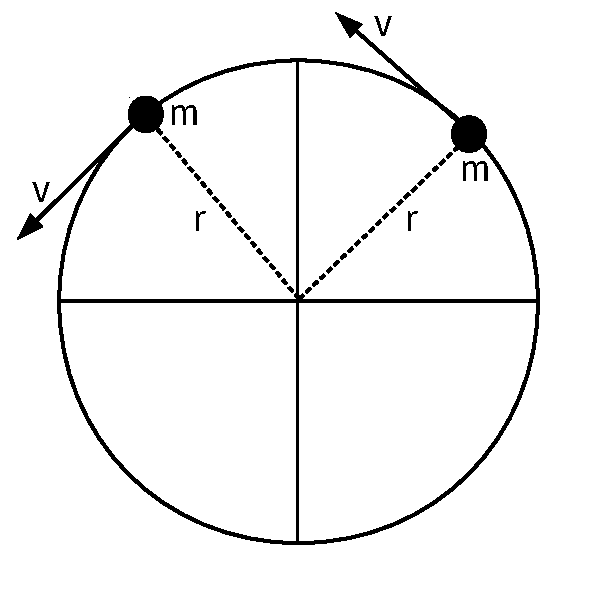
\includegraphics[width=0.2\textwidth]{rotate.pdf}
\end{figure}
\end{enumerate}
\end{document}